\documentclass[11pt]{article}

\usepackage[margin=1in]{geometry}
\usepackage{amsmath, amssymb, enumitem, indentfirst, graphicx, float, comment}
\usepackage[style=numeric]{biblatex}

\graphicspath{ {images/} }

\addbibresource{sources.bib}

\setlength{\parindent}{2em}
\setlength{\parskip}{1em}

\begin{document}
\section*{Topics/Purpose}
For this project, I'll build a very simple game using OpenGL. In the game, the player will start off on a floating platform. His objective would be to jump from one platform to the next, to eventually reach the end. The faster he reaches the end, the higher his score.

The platforms aren't necessarily stationary. They can move side to side. They can also fall if the player does not jump off within a certain amount of time. A level consists of a sequence of platforms. Each level is stored on the disk in some file format. I'll try to leverage Lua to parse and load the levels into the game program.

\begin{figure}[H]
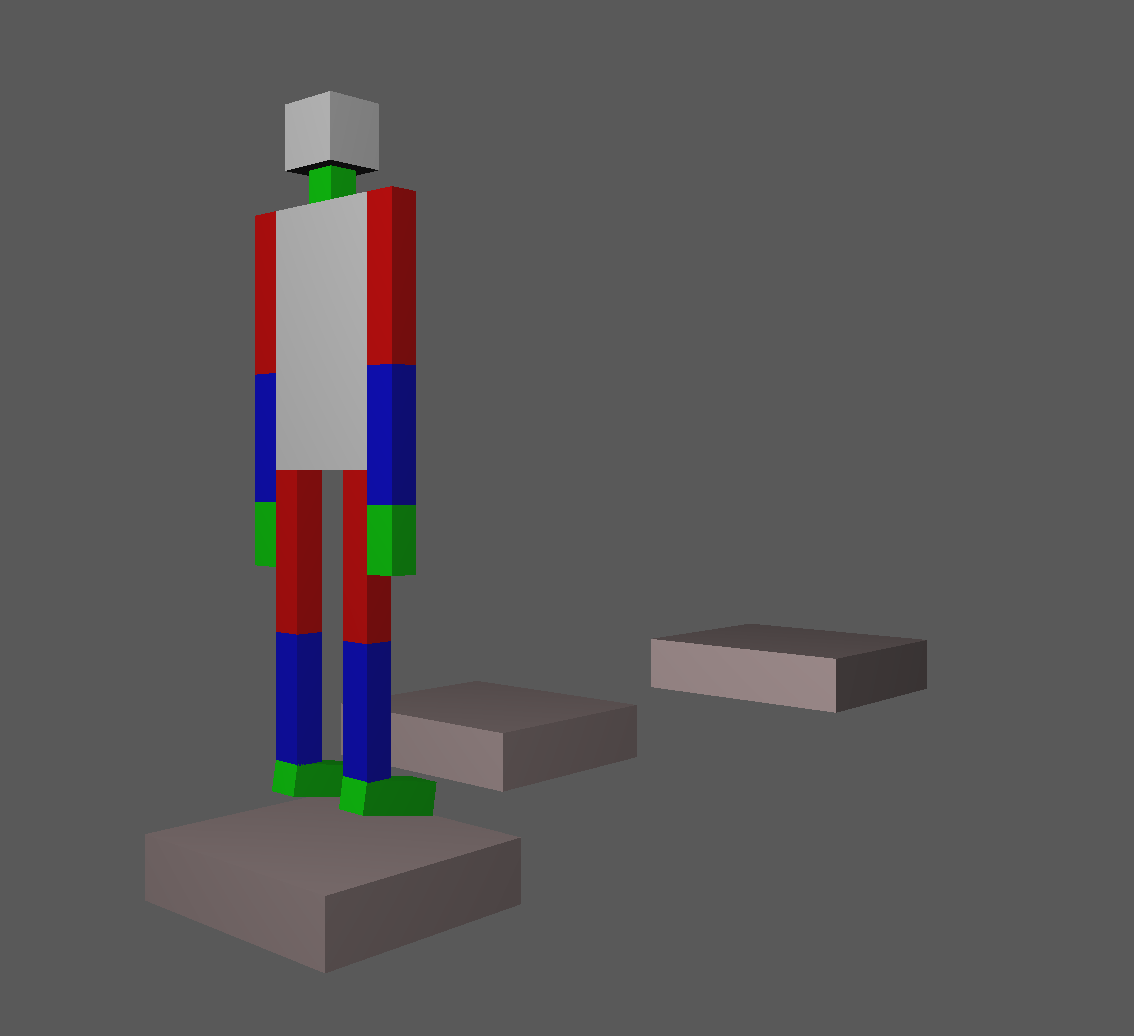
\includegraphics[width=8cm]{screenshot}
\centering
\caption{A first draft screenshot of the player standing on a platform.}
\end{figure}
\section*{Technical Outline}
\subsection*{Texture Mapping}
The platforms for this game will look like dirt or like stones. To achieve this affect, texture mapping will be employed. The algorithm for texture mapping is fairly simple.

A texture is simply a 2 or 1 dimensional array of values. Each value in the texture is referred to as a texture element or a \textit{textel}. To do texture mapping, one first creates a texture for each object. This can be achieved by creating images and loading them into the program. Then, you need to indicate how the texture will be applied to each fragment, given the fragment's original colour and alpha, and the textel's colour and alpha. There's six different approaches for this: \verb|GL_ADD|, \verb|GL_MODULATE|, \verb|GL_DECAL|, \verb|GL_BLEND|, \verb|GL_REPLACE|, and \verb|GL_COMBINE|. Each is described in \cite{texture-map-fn}. Finally, we enable texture mapping and draw the scene, specifying both the texture and the geometric coordinates. The texture coordinate will be a two tuple $(x, y)$ where $x,y \in [0, 1]$ because the texture will be a 2d array. The geometric coordinate will be a three tuple.

In texture mapping, the fragment being textured could map to an area greater than one texture element. In this case, of these many texture elements, one must be selected or generated for the fragment. Of the 6 algorithms that exist to select the texture element, one can be chosen by writing to \verb|GL_TEXTURE_MIN_FILTER| using the \verb|glTexParameteri| function. On the other extreme, the fragment being textured could also map to an area smaller than one texture element. There are two algorithms to handle this case: \verb|GL_NEAREST|, and \verb|GL_LINEAR|. One must be selected by writing to \verb|GL_TEXTURE_MAG_FILTER|. The general details of these algorithms are documented in \cite{gl-tex-parameter}.

\subsection*{Animation}
For animating the puppet movement in this game, I'll use a technique called key-framing. The puppet is represented as a hierarchical 3d model consisting of \verb|JointNode|s, \verb|GeometryNode|s, and \verb|SceneNode|s. I'll define a key-frame as a mapping from a \verb|JointNode| to position and angle. Then, an animation is consists of a sequence of key-frames, each with an associated timestamp. To run the animation, one simply looks at the current time to find the current and the next key-frame. Then, based on the current time, the position and the angle of the joint is interpolated before the model is finally rendered on to the screen.

There can be several different types of animations, two of which are running and jumping. Therefore, I'll need to come up with a way to store the animations. Most likely, the animations will be stored inside a Lua script or a JSON file. I'll also need to implement a number of extra classes to build the animations. The \verb|Animation| class will be the sequence of \verb|KeyFrame| objects. Given a time $t$, the animation class will return a frame which contains the transformations of all the joints. The \verb|KeyFrame| class will be a struct containing a joint's name, its angle, and its position. Finally, there will be class to manage the current time and render the frames returned by the \verb|Animation| instance. Most likely, this will just be the \verb|A5| class.

For this objective, I'll start by consulting \cite{interactive-computer-graphics} to see how best to interpolate between key-frames.

\subsection*{Physics Engine}
Since the player will be jumping from one platform to the next, there will need to exist some sort of physics engine to enable this movement. Within the game, I'll keep a track of the player's current position, acceleration, and velocity in \verb|vec3| objects. Every time we re-render the player, I'll advance the timeline in the physics engine, which will compute, based on the player's current position, current velocity, current acceleration, what his next position and velocity will be. My physics engine will be parameterized to accept the gravitational constant $g$ and also a constant $b$, which will be used in $F_d = -bv$ to determine the amount of drag experienced by the player when he jumps from one platform to the next.

\subsection*{Collisions}
In a manner similar to how bounding volumes were implemented in A4, I'll create axis-aligned bounding volumes for each game object. There will be mainly two types of game objects: the player, and blocks. It's trivial to compute the bounding volume of the blocks since they're simply rectangular prisms. For the puppet, since it's a hierarchical model, I'll have to recursively visit every node in the hierarchy to determine the overall size of the puppet. Once the dimensions of the puppet have been calculated, they will be combined with the puppet's location to create its bounding volume. The dimensions can be calculated when the puppet is first parsed from the Lua file.

Suppose the bounding volume for an object $A$ is specified as $\{X_{min}, Y_{min}, Z_{min}, X_{max}, Y_{max}, Z_{max}\}$, then to check if this bounding volume intersects with the bounding volume of another object $B$, we need to check the following:

\begin{align*}
Intersects_x &= A.X_{min} \leq B.X_{max} \land B.X_{min} \leq A.X_{max} \\
Intersects_y &= A.Y_{min} \leq B.Y_{max} \land B.Y_{min} \leq A.Y_{max} \\
Intersects_z &= A.Z_{min} \leq B.Z_{max} \land B.Z_{min} \leq A.Z_{max} \\
Intersects &= Intersects_x \land Intersects_y \land Intersects_z
\end{align*}

In my game, there will be both static and dynamic collisions. The static collisions will be a special case of the dynamic collisions. There will be dynamic collisions because both the platforms and the player can move. The main source I'll consult for 3d collisions would be \cite{mdn3dcd}.

\subsection*{Motion Blur}
Modern graphics hardware gives access to an accumulation buffer. This is essentially the same as the colour buffer but it cannot be written to directly. Instead, OpenGL makes available 6 operations that developers can perform on the accumulation buffer. First, you can call \verb|glAccum(GL_LOAD, value)| to copy the contents of the colour buffer multiplied by \verb|value| into the accumulation buffer. Second, you can call \verb|glAccum(GL_ACCUM, value)| to add the contents of the accumulation buffer to the contents of the colour buffer multiplied by \verb|value| to the accumulation buffer. Third, you can call \verb|glAccum(GL_RETURN, value)| to copy the contents of the accumulation buffer multiplied by \verb|value| to the colour buffer. These three operations are all that's required to implement motion blur.

Instead of calling \verb|glSwapBuffers()| in every turn of the OpenGL rendering loop (thereby rendering the image to the screen), you instead add the colours scaled by $\frac{1}{n}$ to the accumulation buffer. Then after the $n$'th iteration, you write copy the colours from the accumulation buffer to the colour buffer and call \verb|glSwapBuffers()| to show the blurred image on the screen. On the first iteration, you'd directly copy the colours from the colour buffer scaled by $\frac{1}{n}$, which would reset the accumulation buffer. The algorithm is more succinctly described in \cite{wikibooks-motion-blur}. 

\subsection*{Shadow Mapping}
Since this game has light sources, shadows are also necessary to produce realistic imagery. There's no perfect algorithm to implement shadows---it hasn't yet been invented. So, most games today rely on shadow approximation techniques to get decent results. The approximation technique I'll be employing in this project is called Shadow Mapping. The general algorithm is described below.

Suppose that we have a singular light source and a world consisting of objects. Then, it's possible to determine whether each point in the world should be in a shadow or not. The scene is visualized in Figure 2.

\begin{figure}[H]
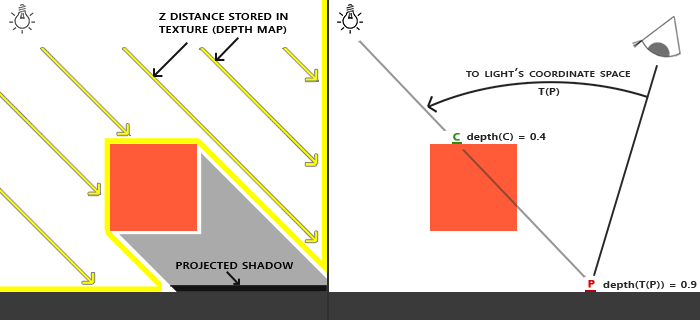
\includegraphics[width=8cm]{shadow_mapping_theory_spaces}
\centering
\caption{An illustration of how to produce shadows using OpenGL's depth buffer\cite{shadow-map-learn-opengl}.}
\end{figure}

The algorithm for shadow mapping is really simple. For each point $P$, we view it from the perspective of the light source. In this coordinate frame, we render the entire scene, using the z-buffer algorithm. This builds a depth buffer, which lets us know for each $(x, y)$, the depth of the closest point to the light source.

After the depth buffer is obtained, we render the scene properly from the perspective of the actual camera. For each fragment, we transform it to the coordinate frame of the light source. Then, before rendering the fragment, we look in the depth buffer at that fragment's transformed $(x, y)$. If the fragment we're trying to render has a depth greater than the depth stored in the depth buffer at point $(x, y)$, then the fragment must be in a shadow. Hence, we render the fragment with darker colour. If the fragment's z value is equal to the z value stored at the depth buffer, then it must be directly illuminated by the light source. In that case, we render it normally.  

The actual implementation of the Shadow Map is a bit more nuanced. In implementing the algorithm, one can run into problems such as blocky shadows, Shadow acne, or peter panning. None of these problems are insurmountable, however. The details of the algorithm's implementation are discussed in \cite{shadow-map-learn-opengl}, which I'll use as my primary source to implement the Shadow Mapping in my game.

\printbibliography
\section*{Objectives}
\begin{enumerate}
\item Modeling the Scene.
\item UI.
\item Texture mapping.
\item Animation.
\item Static collisions.
\item Dynamic collisions.
\item Synchronized sound.
\item Physics Engine.
\item Motion blur.
\item Shadows using shadow maps.
\end{enumerate}
\end{document}
